\section{Visualization}
\subsection{SFC for HyperGraph}
Existing hypergraph visualization approaches can be divided into three categories~\cite{fischer2021hypergraphsurvey}: 
(1) node-link-based, (2) timeline-based, and (3) matrix-based approaches.
We first exclude timeline-based approaches because we do not consider temporal attributes of the data in the system.
As for matrix-based approaches, although they are known for their visual scalability, they are not suitable for our system because of their lack of support for visualizing hierarchical clusters and user interactions.
In the design guidelines proposed by Abdelaal et.al.~\cite{abdelaal2022network} in a recent network visualization evaluation study, node-link-based approaches are recommended when:
(1) tasks involve the identification of network clusters, and (2) the network is sparse.
Condition (1) is fulfilled as explained in~\autoref{sec: design_rationale}, and (2) is guaranteed by the main participant extraction process described in~\autoref{sec: participant_extraction}. 
Therefore, we decided to use node-link-based approaches for our system.

Although there are a variety of node-link-based approaches for hypergraph visualization, we find the extra-node representation proposed by Ouvrard et.al.~\cite{ouvrard2017hypergraph} most flexible and intuitive.
An extra-node representation improves existing clique-expansion of hypergraphs by adding extra nodes to represent hyperedges. 
The extra-node representation effectively transforms the hypergraph visualization problem into a bipartite graph visualization problem.
After that, any node-link-based graph visualization method can be applied.

In our system, we use the space-filling curve (SFC) layout method to layout the extra-node representation of the hypergraph.
The SFC layout method uses pre-computed clustering to order nodes in a sequence and then applies a space-filling curve on the node sequence to map it to a two-dimensional screen space~\cite{muelder2008sfc}.
SFC approaches are known for their efficiency and aesthetics in visualizing large graphs~\cite{ma2013largegraph}.
After the preprocessing and modeling stage described in~\autoref{sec: methodology}, we have two hypergraphs: the article hypergraph $H_A$ and the participant hypergraph $H_P$, each having its hierarchical cluster.
Combining the extra-node representation and SFC layout, we visualize the article hypergraph $H_A$ and the participant hypergraph $H_P$ as two separate SFCs, as shown in~\autoref{fig: sfc}.

Specifically, we divide the layout space into two parts: the peripheral and the center area.
For the peripheral area, we concatenate four generalized Hilbert (Gilbert) curves~\cite{gilbert}.
Through rotation and flipping, the start and end curve points for neighboring Gilbert curves are concatenated smoothly, as shown in~\autoref{fig: gilbert}.
The use of concatenated Gilbert curves allows us to fill the peripheral space while having the benefits of SFC layouts.
For the center area, we use a simple Gosper curve to layout the nodes.
The resulting visualization looks similar to GosperMap~\cite{auber2013gospermap}.
However, the curve to be used for the center area is flexible since it is guaranteed to be a squared region.
Also, the interactions to support the exploration and reorganization of the dataset are the main focus of the system, which is also not limited to any specific curve.

After the curves are generated, we can apply the curves on the node sequences to generate the two-dimensional layout.
We chose to put the article hypergraph in the center area because the articles are the main analysis targets for the user.
Consequently, the participant hypergraph is put in the peripheral area.
\subparagraph{Spacing Strategy}
We employ a simple spacing strategy.

\subsection{Borders and Labeling}
Labeling the clusters is essential for users to explore the dataset.
When using SFC layouts, the automatic labeling process is challenging because the shape of the clusters can be irregular.
After applying the SFC layout, we use a concave hull algorithm~\cite{park2012concavehull} to generate an approximation polygon for each cluster.
The polygons are used to generate borders and calculate label positions for the clusters.
\subparagraph{Borders} 
The borders are generated by applying a smoothing algorithm on the polygons.
For Gosper curves, we use the polygon as control points to generate a cubic basis spline as the border.
For Gilbert curves, we use a similar approach but with a cubic Bezier curve.
More specifically, for each pair of consecutive control points, we use a smoothing factor to interpolate the control point.
This results in a sketchy style at the borders.
Two examples are given in~\autoref{fig: borders}.
\subparagraph{Labeling}
\begin{figure}%
    \centering
    \subfloat[\centering One Gilbert curve]{{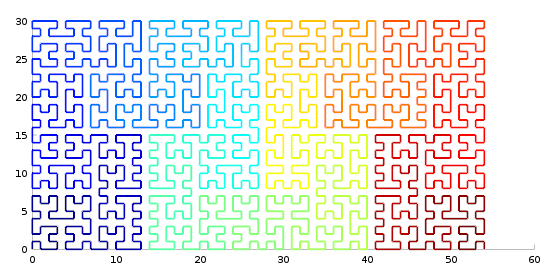
\includegraphics[width=5cm]{gilbert} }}%
    \qquad
    \subfloat[\centering Four concatenated Gilbert curves]{{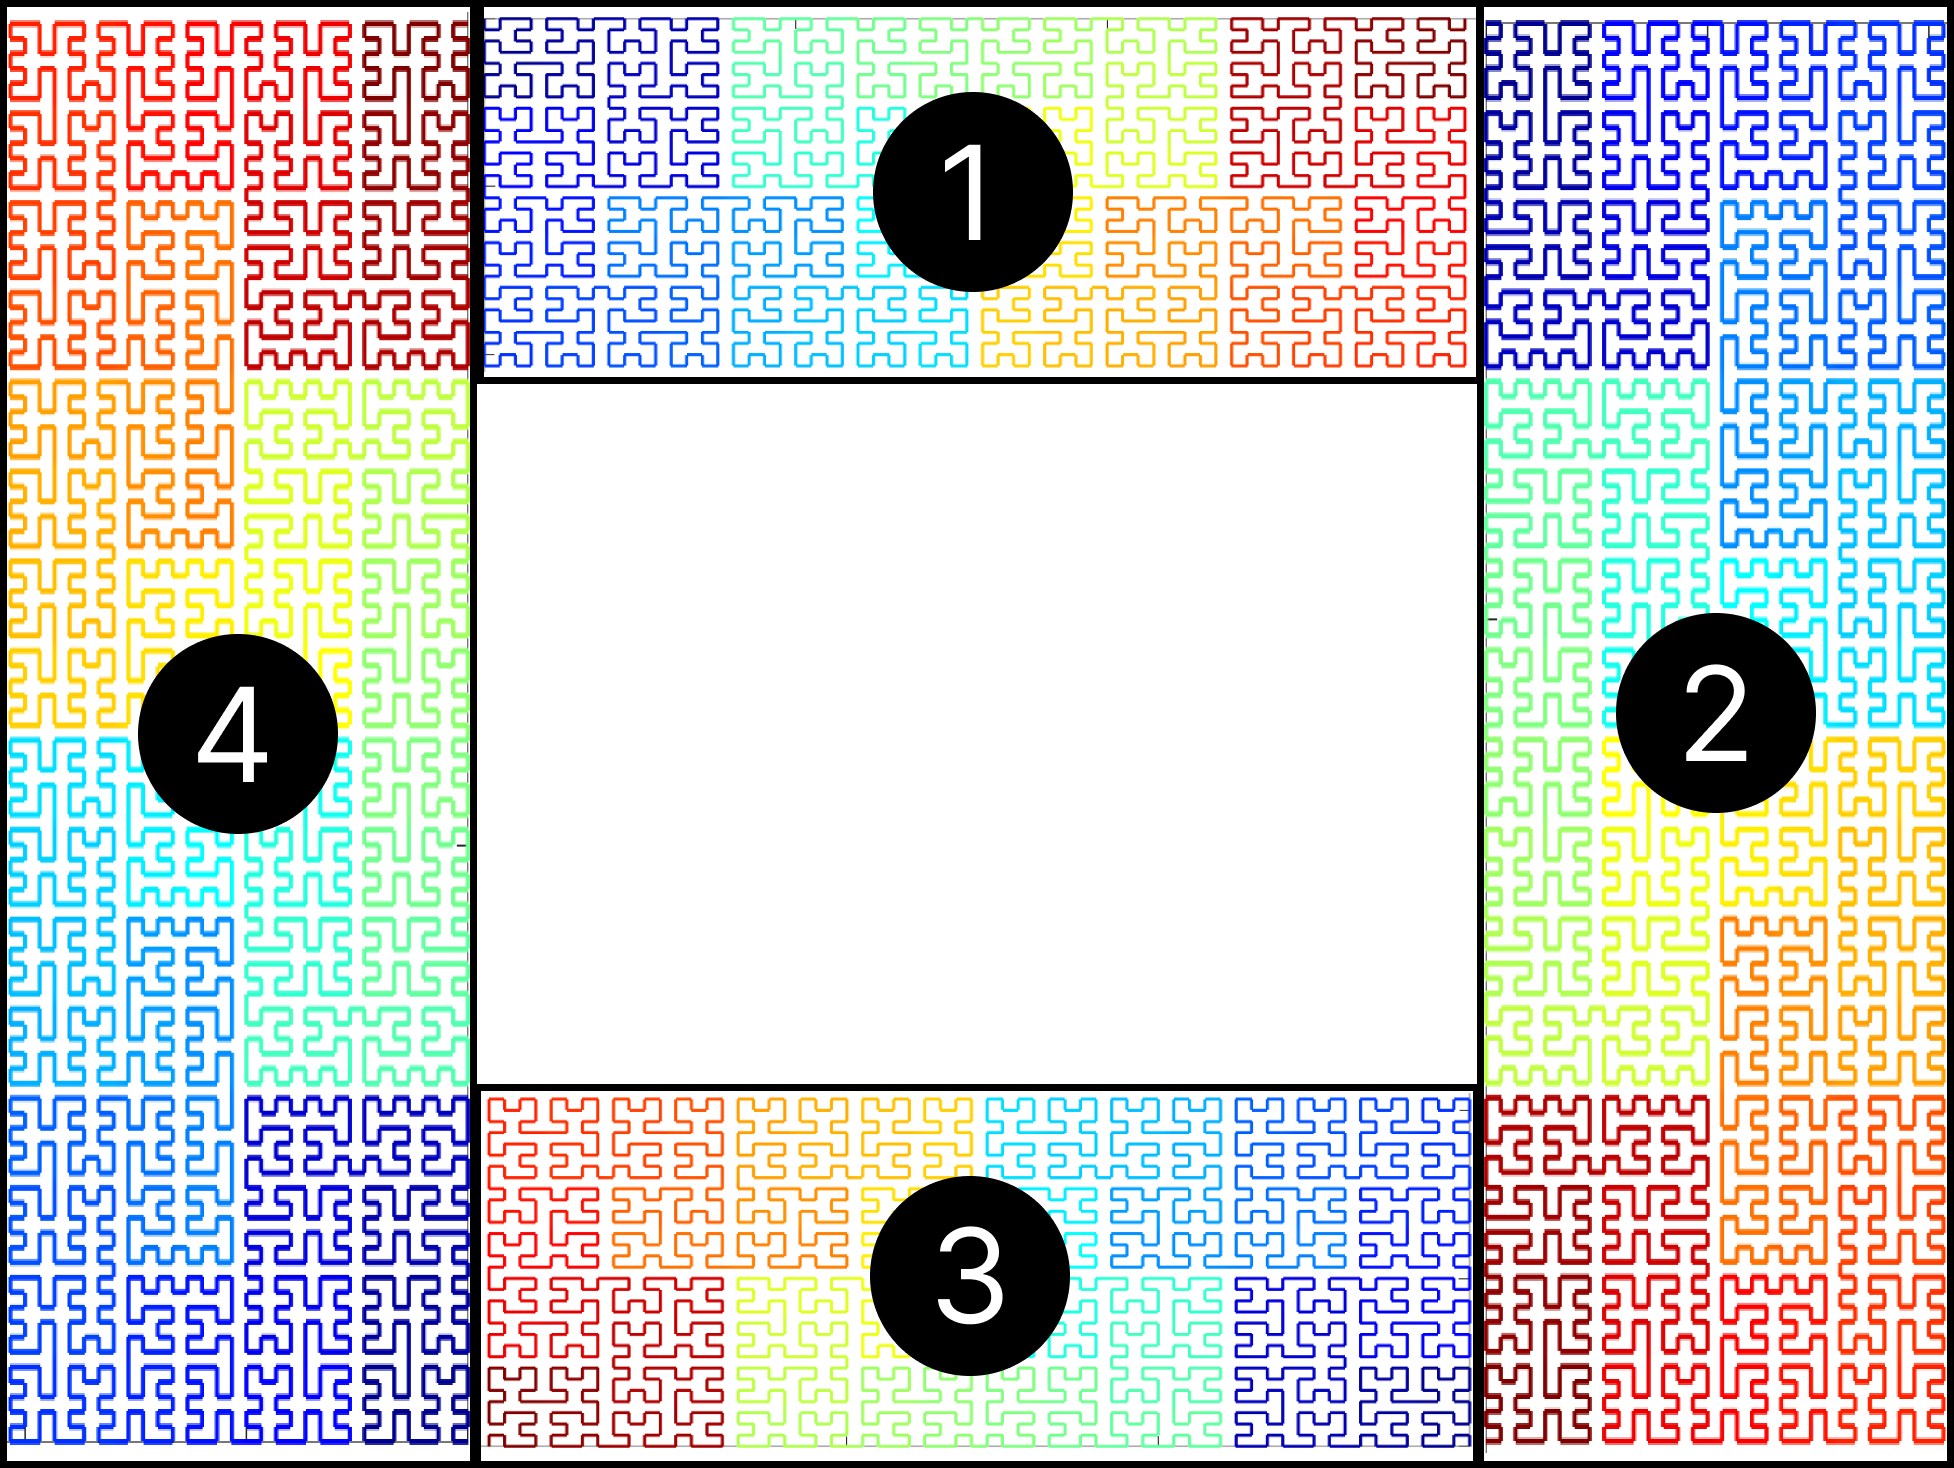
\includegraphics[width=5cm]{concatenated_gilbert} }}%
    \caption{
        Illustration of concatenating Gilbert curves. 
        The color indicates the traverse direction of Gilbert curves: start with dark blue and end with dark red.
    }%
    \label{fig: gilbert}%
\end{figure}
\begin{figure}%
    \centering
    \subfloat[\centering ]{{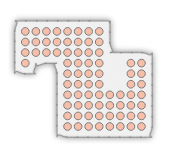
\includegraphics[width=5cm]{example_gilbert_border} }}%
    \qquad
    \subfloat[\centering ]{{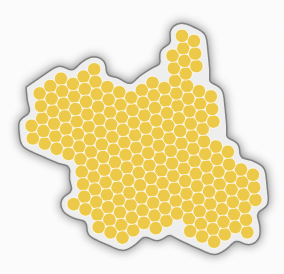
\includegraphics[width=5cm]{example_gosper_border} }}%
    \caption{(a) An example of Gilbert cluster border (b) An example of Gosper cluster borders}%
    \label{fig: borders}%
\end{figure}
% \begin{figure}
% \centering
% \begin{subfigure}{.5\textwidth}
% \centering
% 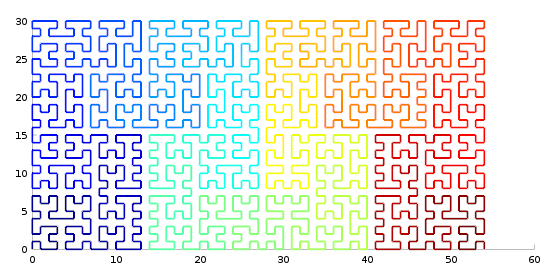
\includegraphics[width=.4\linewidth]{gilbert}
% \caption{A subfigure}
% \end{subfigure}%
% \begin{subfigure}{.5\textwidth}
% \centering
% 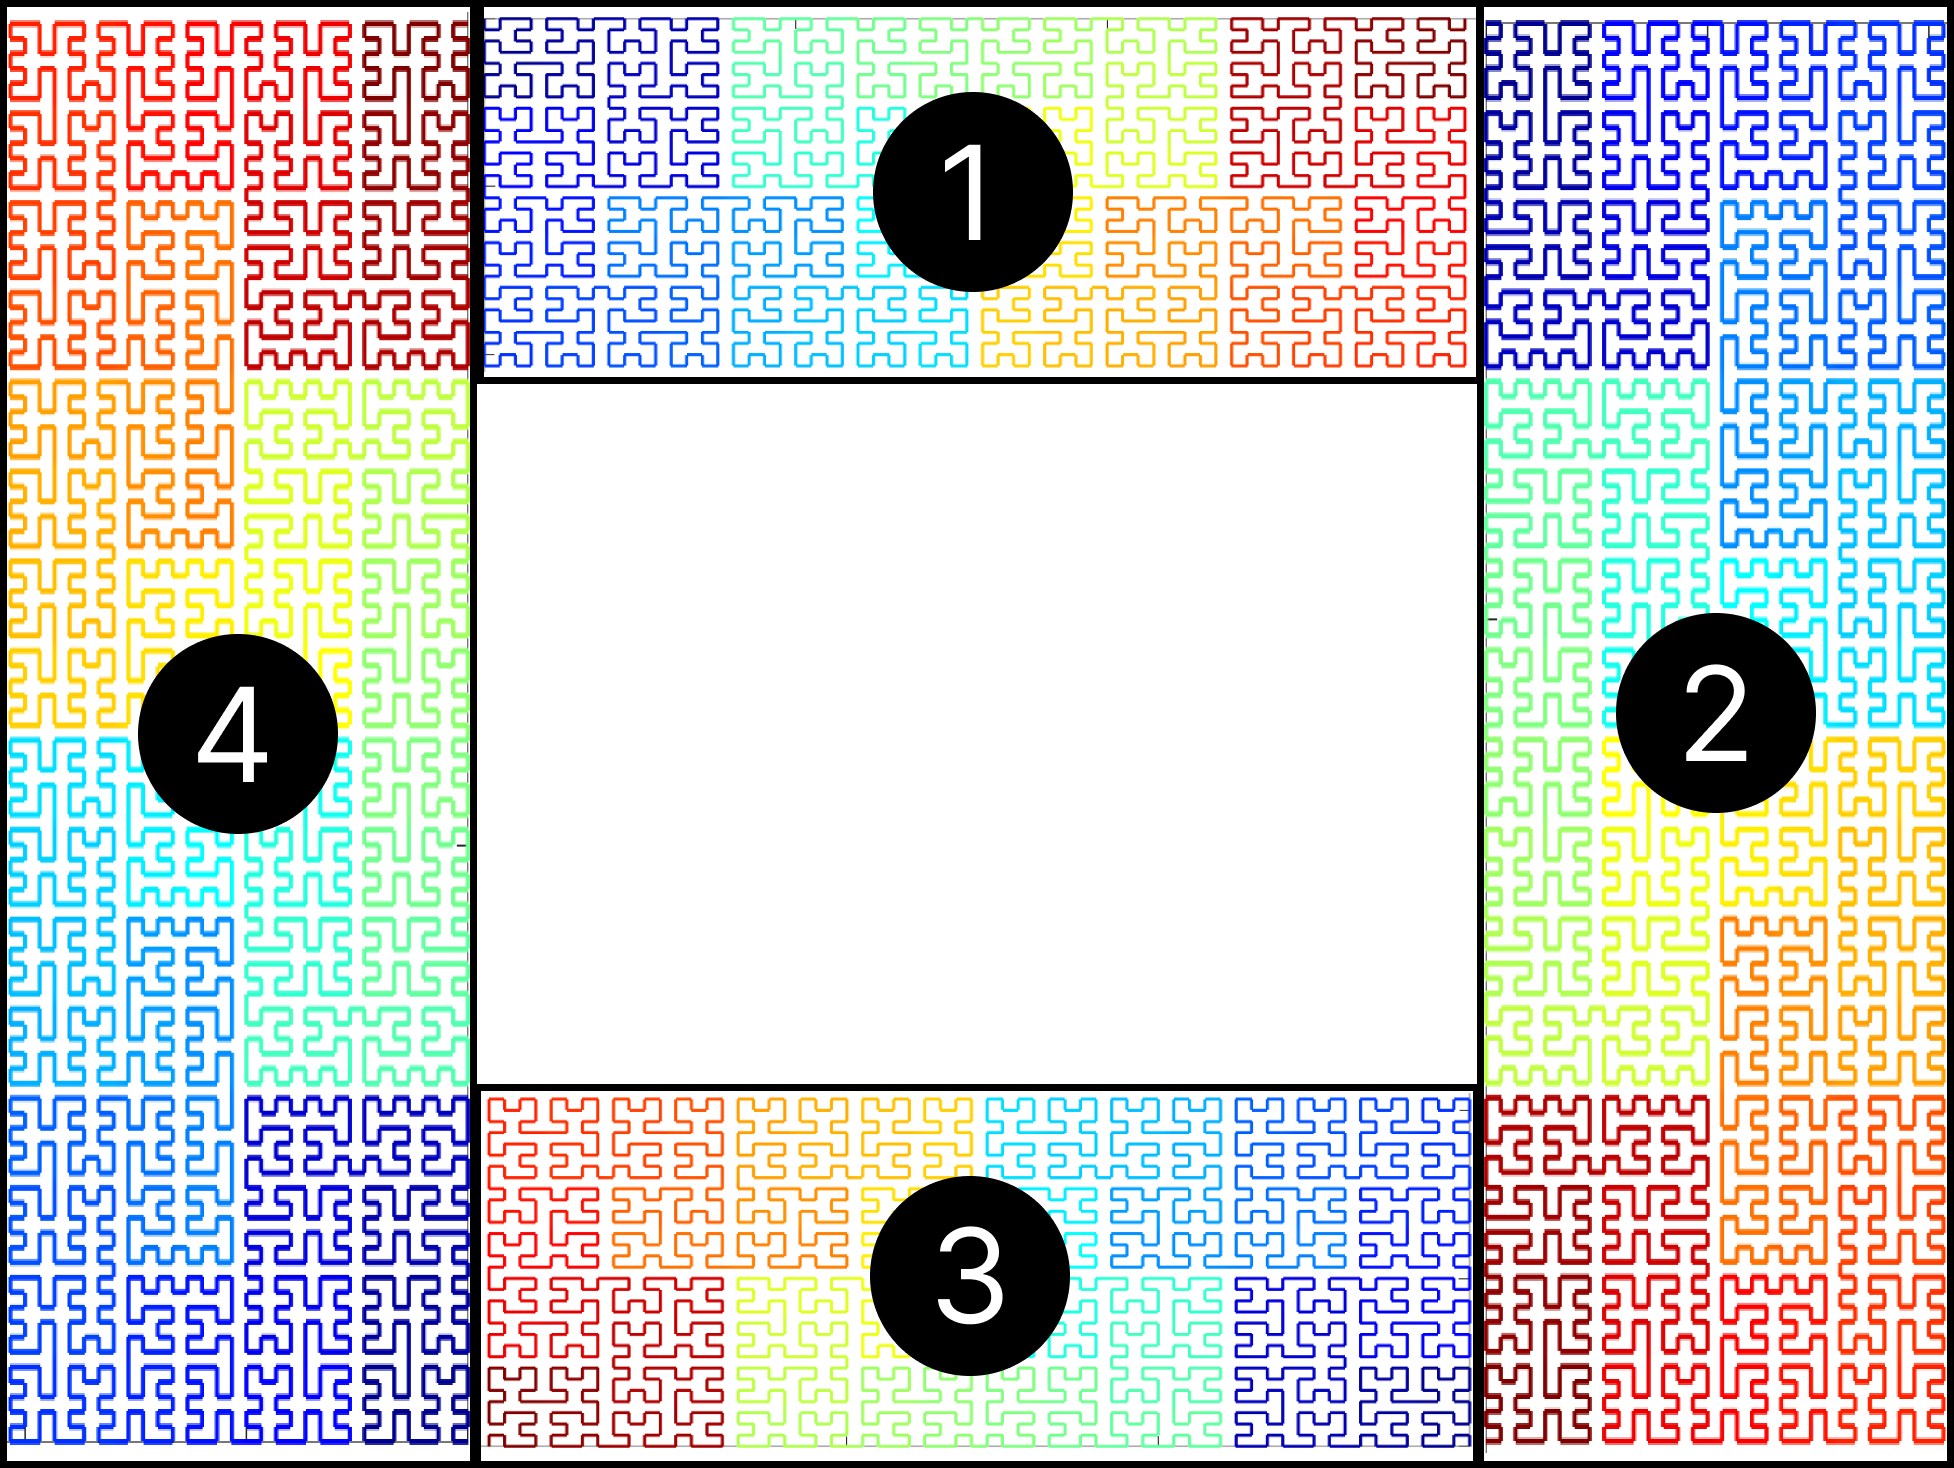
\includegraphics[width=.4\linewidth]{concatenated_gilbert}
% \caption{Another subfigure}
% \end{subfigure}
% \caption{A figure with two subfigures}
% \label{fig:gilbert}
% \end{figure}



